\section{Exemplos de simulações}

Nesta seção é possível observar algumas simulações feitas afim de exemplificar o PCP e assim verificar se a implementação do mesmo está correta.

\subsection{Teste 1}
\subsubsection{Configurações}
\begin{table}[H]
\centering
\caption{\em Tarefas.}
\vspace{0.1cm}
\begin{tabular}{c||c|c|c|c|c|c|c}
 
Parâmetros & $\tau_1$ & $\tau_2$ & $\tau_3$ & $\tau_4$ & $\tau_5$ & $\tau_6$ & $\tau_7$\\ 
\hline 
                          
$a_i$ & 0 & 0 & 0 & 2 & 3 & 5 & 7\\ 
$C_i$ & 4 & 2 & 4 & 3 & 6 & 2 & 1\\ 
$D_i$ & 30 & 32 & 36 & 33 & 30 & 40 & 31\\
$P_i$ & 1 & 2 & 3 & 5 & 4 & 7 & 6
 
\end{tabular}
\end{table}

\begin{table}[H]
\centering
\caption{\em Semáforo.}
\vspace{0.1cm}
\begin{tabular}{c||c|c|c||c|c|c||c|c|c}
 
Tarefas & $Sa_1$ & $Sa_C1$ & Status 1 & $Sa_2$ & $Sa_C2$ & Status 2 & $Sa_3$ & $Sa_C3$ & Status 3\\ 
\hline 
                          
$\tau_1$ & 0 & 0 & 2 & 3 & 2 & 0 & 0 & 0 & 2\\ 
$\tau_2$ & 1 & 1 & 0 & 0 & 0 & 2 & 0 & 0 & 2\\
$\tau_3$ & 0 & 2 & 1 & 2 & 3 & 0 & 0 & 1 & 0\\
$\tau_4$ & 0 & 0 & 2 & 0 & 0 & 2 & 1 & 1 & 0\\
$\tau_5$ & 0 & 0 & 2 & 1 & 1 & 0 & 0 & 0 & 2\\
$\tau_6$ & 0 & 0 & 2 & 2 & 1 & 0 & 0 & 0 & 2\\
$\tau_7$ & 0 & 0 & 2 & 0 & 0 & 2 & 0 & 0 & 2
 
\end{tabular}
\end{table}

\subsubsection{Resultado da Simulação}

\begin{figure}[H]
	\centering
	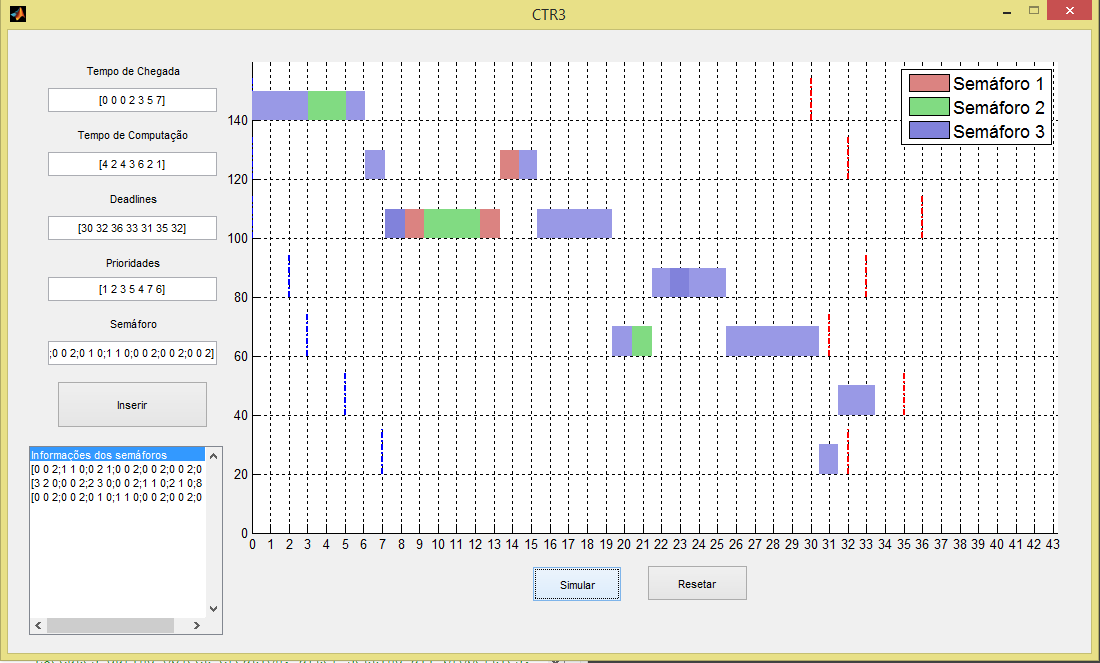
\includegraphics[keepaspectratio,width=1\textwidth]{img/teste1.png}
\end{figure}



\subsection{Teste 2}
\subsubsection{Configurações}
\begin{table}[H]
\centering
\caption{\em Tarefas.}
\vspace{0.1cm}
\begin{tabular}{c||c|c|c|c|c}
 
Parâmetros & $\tau_1$ & $\tau_2$ & $\tau_3$ & $\tau_4$ & $\tau_5$\\ 
\hline 
                          
$a_i$ & 0 & 0 & 3 & 5 & 7\\ 
$C_i$ & 4 & 2 & 6 & 3 & 2\\ 
$D_i$ & 6 & 11 & 20 & 30 & 25\\
$P_i$ & 1 & 2 & 4 & 6 & 5
 
\end{tabular}
\end{table}

\begin{table}[H]
\centering
\caption{\em Semáforo.}
\vspace{0.1cm}
\begin{tabular}{c||c|c|c||c|c|c}
 
Tarefas & $Sa_1$ & $Sa_C1$ & Status 1 & $Sa_2$ & $Sa_C2$ & Status 2\\ 
\hline 
                          
$\tau_1$ & 0 & 0 & 2 & 3 & 2 & 0 \\ 
$\tau_2$ & 1 & 1 & 0 & 0 & 0 & 2 \\
$\tau_3$ & 0 & 0 & 2 & 1 & 1 & 0 \\
$\tau_4$ & 0 & 0 & 2 & 2 & 1 & 0 \\
$\tau_5$ & 0 & 0 & 2 & 1 & 2 & 0 

\end{tabular}
\end{table}

\subsubsection{Resultado da Simulação}

\begin{figure}[H]
	\centering
	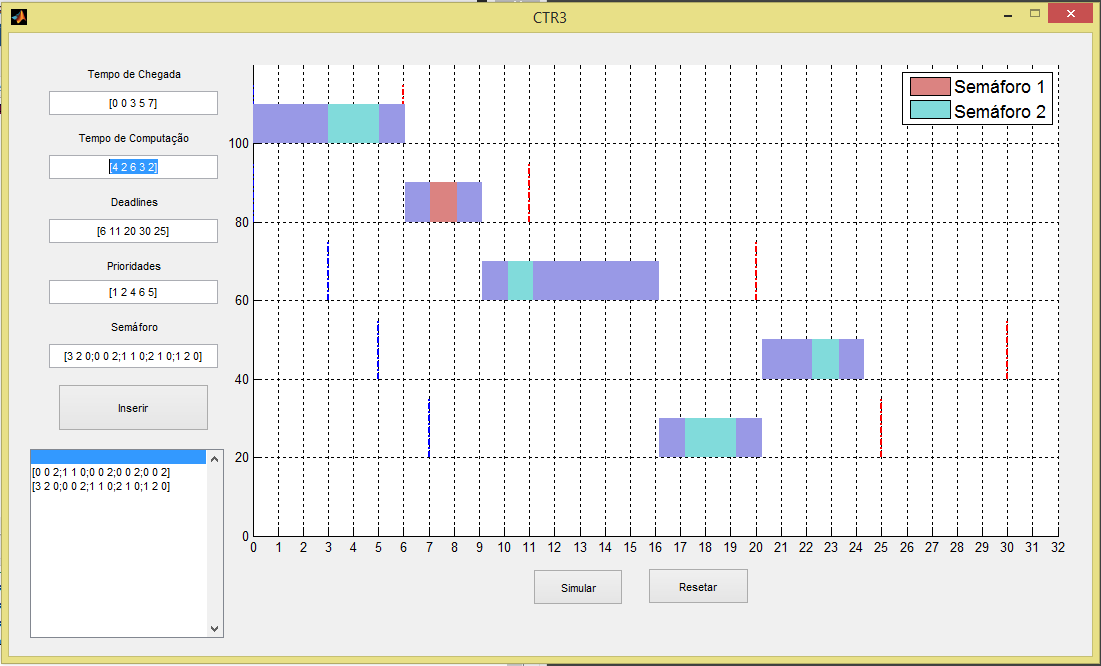
\includegraphics[keepaspectratio,width=1\textwidth]{img/teste2.png}
\end{figure}



\subsection{Teste 3}
\subsubsection{Configurações}
\begin{table}[H]
\centering
\caption{\em Tarefas.}
\vspace{0.1cm}
\begin{tabular}{c||c|c|c|c|c}
 
Parâmetros & $\tau_1$ & $\tau_2$ & $\tau_3$ & $\tau_4$ & $\tau_5$\\ 
\hline 
                          
$a_i$ & 0 & 0 & 3 & 5 & 7\\ 
$C_i$ & 4 & 2 & 6 & 3 & 3\\ 
$D_i$ & 6 & 13 & 20 & 29 & 25\\
$P_i$ & 1 & 2 & 4 & 6 & 5
 
\end{tabular}
\end{table}

\begin{table}[H]
\centering
\caption{\em Semáforo.}
\vspace{0.1cm}
\begin{tabular}{c||c|c|c}
 
Tarefas & $Sa_1$ & $Sa_C1$ & Status 1\\ 
\hline 
                          
$\tau_1$ & 3 & 2 & 0\\ 
$\tau_2$ & 1 & 4 & 0\\
$\tau_3$ & 1 & 1 & 0\\
$\tau_4$ & 2 & 1 & 0\\
$\tau_5$ & 1 & 2 & 0
 
\end{tabular}
\end{table}

\subsubsection{Resultado da Simulação}

\begin{figure}[H]
	\centering
	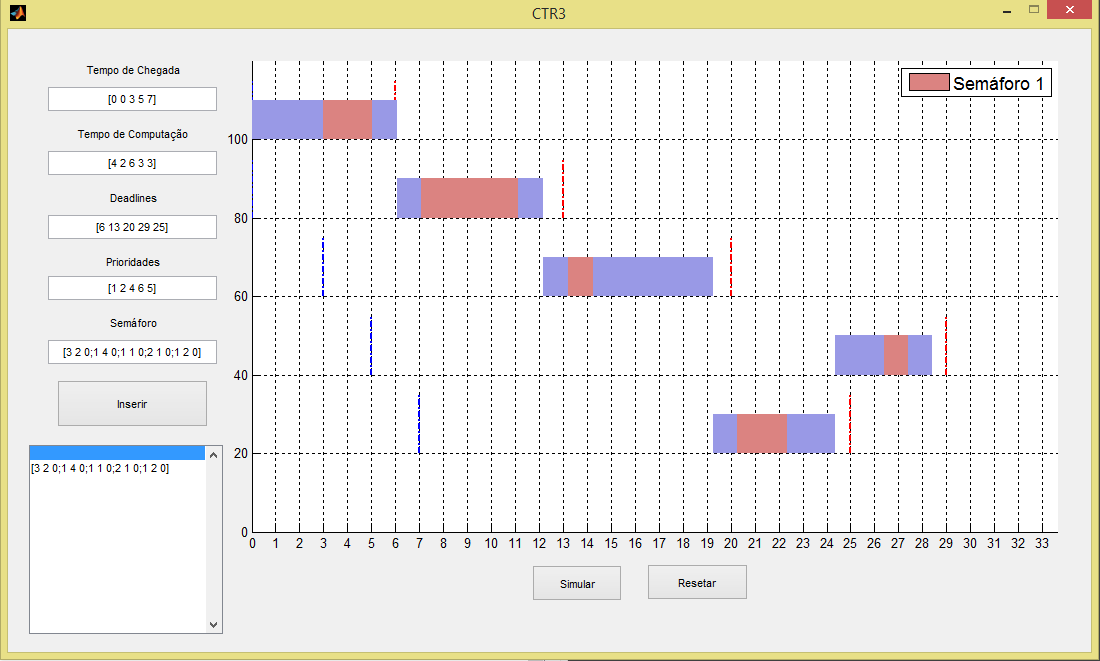
\includegraphics[keepaspectratio,width=1\textwidth]{img/teste3.png}
\end{figure}



\subsection{Teste 4}
\subsubsection{Configurações}
\begin{table}[H]
\centering
\caption{\em Tarefas.}
\vspace{0.1cm}
\begin{tabular}{c||c|c|c|c|c|c|c|c}
 
Parâmetros & $\tau_1$ & $\tau_2$ & $\tau_3$ & $\tau_4$ & $\tau_5$ & $\tau_6$ & $\tau_7$ & $\tau_8$\\ 
\hline 
                          
$a_i$ & 1 & 0 & 0 & 0 & 0 & 0 & 0 & 0\\ 
$C_i$ & 4 & 2 & 7 & 5 & 6 & 3 & 3 & 9\\ 
$D_i$ & 30 & 32 & 36 & 33 & 37 & 43 & 45 & 55\\
$P_i$ & 1 & 2 & 3 & 5 & 4 & 7 & 6 & 8
 
\end{tabular}
\end{table}


\begin{table}[H]
\centering
\caption{\em Semáforos 1.}
\vspace{0.1cm}
\begin{tabular}{c||c|c|c||c|c|c}
 
Tarefas & $Sa_1$ & $Sa_C1$ & Status 1 & $Sa_2$ & $Sa_C2$ & Status 2\\ 
\hline 
                          
$\tau_1$ & 0 & 0 & 2 & 3 & 2 & 0\\ 
$\tau_2$ & 1 & 1 & 0 & 0 & 0 & 2\\
$\tau_3$ & 0 & 2 & 1 & 2 & 3 & 0\\
$\tau_4$ & 0 & 0 & 2 & 0 & 0 & 2\\
$\tau_5$ & 0 & 0 & 2 & 1 & 1 & 0\\
$\tau_6$ & 0 & 0 & 2 & 2 & 1 & 0\\
$\tau_7$ & 0 & 0 & 2 & 1 & 2 & 0\\
$\tau_8$ & 0 & 0 & 2 & 0 & 0 & 2

\end{tabular}
\end{table}


\begin{table}[H]
\centering
\caption{\em Semáforos 2.}
\vspace{0.1cm}
\begin{tabular}{c||c|c|c||c|c|c}
 
Tarefas & $Sa_3$ & $Sa_C3$ & Status 3 & $Sa_4$ & $Sa_C4$ & Status 4\\ 
\hline 
                          
$\tau_1$ & 0 & 0 & 2 & 0 & 0 & 2\\ 
$\tau_2$ & 0 & 0 & 2 & 0 & 0 & 2\\
$\tau_3$ & 0 & 1 & 0 & 0 & 0 & 2\\
$\tau_4$ & 1 & 1 & 0 & 0 & 0 & 2\\
$\tau_5$ & 0 & 0 & 2 & 0 & 0 & 2\\
$\tau_6$ & 0 & 0 & 2 & 0 & 0 & 2\\
$\tau_7$ & 0 & 0 & 2 & 0 & 0 & 2\\
$\tau_8$ & 0 & 0 & 2 & 3 & 1 & 0

\end{tabular}
\end{table}

\subsubsection{Resultado da Simulação}

\begin{figure}[H]
	\centering
	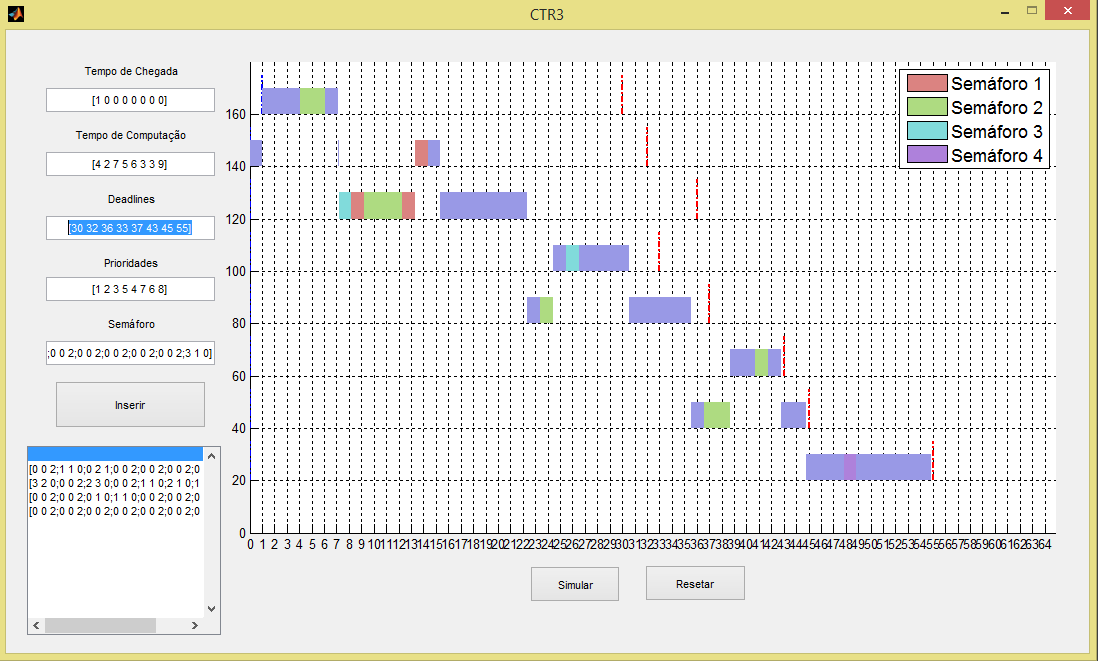
\includegraphics[keepaspectratio,width=1\textwidth]{img/teste4.png}
\end{figure}